\documentclass{report}
% Include all project wide packages here.
\usepackage{fullpage}
\usepackage[style=ieee]{biblatex}
\usepackage[dutch]{babel}

\renewcommand{\familydefault}{\sfdefault}

\setmainfont[Ligatures=TeX]{Myriad Pro}
\setmathfont{Asana Math}
\setmonofont{Lucida Console}

\usepackage{titlesec, blindtext, color}
\definecolor{gray75}{gray}{0.75}
\newcommand{\hsp}{\hspace{20pt}}
\titleformat{\chapter}[hang]{\Huge\bfseries}{\thechapter\hsp\textcolor{gray75}{|}\hsp}{0pt}{\Huge\bfseries}
\renewcommand{\familydefault}{\sfdefault}
\renewcommand{\arraystretch}{1.2}
\setlength\parindent{0pt}

%For code listings
\definecolor{black}{rgb}{0,0,0}
\definecolor{browntags}{rgb}{0.65,0.1,0.1}
\definecolor{bluestrings}{rgb}{0,0,1}
\definecolor{graycomments}{rgb}{0.4,0.4,0.4}
\definecolor{redkeywords}{rgb}{1,0,0}
\definecolor{bluekeywords}{rgb}{0.13,0.13,0.8}
\definecolor{greencomments}{rgb}{0,0.5,0}
\definecolor{redstrings}{rgb}{0.9,0,0}
\definecolor{purpleidentifiers}{rgb}{0.01,0,0.01}


\lstdefinestyle{csharp}{
language=[Sharp]C,
showspaces=false,
showtabs=false,
breaklines=true,
showstringspaces=false,
breakatwhitespace=true,
escapeinside={(*@}{@*)},
columns=fullflexible,
commentstyle=\color{greencomments},
keywordstyle=\color{bluekeywords}\bfseries,
stringstyle=\color{redstrings},
identifierstyle=\color{purpleidentifiers},
basicstyle=\ttfamily\small}

\lstdefinestyle{c}{
language=C,
showspaces=false,
showtabs=false,
breaklines=true,
showstringspaces=false,
breakatwhitespace=true,
escapeinside={(*@}{@*)},
columns=fullflexible,
commentstyle=\color{greencomments},
keywordstyle=\color{bluekeywords}\bfseries,
stringstyle=\color{bluestrings},
identifierstyle=\color{purpleidentifiers}
}

\lstdefinestyle{vhdl}{
language=VHDL,
showspaces=false,
showtabs=false,
breaklines=true,
showstringspaces=false,
breakatwhitespace=true,
escapeinside={(*@}{@*)},
columns=fullflexible,
commentstyle=\color{greencomments},
keywordstyle=\color{bluekeywords}\bfseries,
stringstyle=\color{redstrings},
identifierstyle=\color{purpleidentifiers}
}

\lstdefinestyle{xaml}{
language=XML,
showspaces=false,
showtabs=false,
breaklines=true,
showstringspaces=false,
breakatwhitespace=true,
escapeinside={(*@}{@*)},
columns=fullflexible,
commentstyle=\color{greencomments},
keywordstyle=\color{redkeywords},
stringstyle=\color{bluestrings},
tagstyle=\color{browntags},
morestring=[b]",
  morecomment=[s]{<?}{?>},
  morekeywords={xmlns,version,typex:AsyncRecords,x:Arguments,x:Boolean,x:Byte,x:Char,x:Class,x:ClassAttributes,x:ClassModifier,x:Code,x:ConnectionId,x:Decimal,x:Double,x:FactoryMethod,x:FieldModifier,x:Int16,x:Int32,x:Int64,x:Key,x:Members,x:Name,x:Object,x:Property,x:Shared,x:Single,x:String,x:Subclass,x:SynchronousMode,x:TimeSpan,x:TypeArguments,x:Uid,x:Uri,x:XData,Grid.Column,Grid.ColumnSpan,Click,ClipToBounds,Content,DropDownOpened,FontSize,Foreground,Header,Height,HorizontalAlignment,HorizontalContentAlignment,IsCancel,IsDefault,IsEnabled,IsSelected,Margin,MinHeight,MinWidth,Padding,SnapsToDevicePixels,Target,TextWrapping,Title,VerticalAlignment,VerticalContentAlignment,Width,WindowStartupLocation,Binding,Mode,OneWay,xmlns:x}
}

%defaults
\lstset{
basicstyle=\ttfamily\small,
extendedchars=false,
numbers=left,
numberstyle=\ttfamily\tiny,
stepnumber=1,
tabsize=4,
numbersep=5pt
}
\addbibresource{../../library/bibliography.bib}

\title{EPO-2: Mid-term Design Report - Routeplanner in C}
\author{Robin Hes}

\begin{document}

\chapter{Routeplanner in C}
\label{ch:route}

Een belangrijk onderdeel van het probleem is het vinden van een pad van begin naar eind.
De mens is vrij gemakkelijk in staat een geschikt pad te onderscheiden, maar onze robot is autonoom en dus moet er een oplossing komen die zelf het beste pad berekent.
Dit zou met de FPGA kunnen, maar de schakeling en rekenkracht die daarvoor benodigd is zou dit vrij complex maken.
Bij het EPO-2-project is er dan ook voor gekozen het pad te laten berekenen door een programma geschreven in de C-programmeertaal.
Dit programma draait op een normale computer.

\section{Eisen}
\label{route-eisen}

We kunnen voor het programma de volgende eisen opstellen:

\begin{itemize}
	\item Het programma moet geschreven zijn in C
	\item Het programma moet de snelste route vinden van punt naar punt over het wedstrijdveld
	\item Het programma moet obstakels (mijnen) kunnen ontwijken (geen onderdeel van eerste opdracht)
	\item Het programma moet door de robot gedetecteerde mijnen kunnen opslaan
\end{itemize}

\section{Ontwerp en implementatie}
\label{sec:ontwerp-impl}

\subsection{Lee}
\label{ssec:lee}

De eerste stap bij het schrijven van zo een programma is het vinden van een geschikt algoritme.
Hiervoor hebben we ons georiënteerd op de vele beschikbare algoritmen.
Uiteindelijk is er door elk van de drie tweetallen binnen D-2 gekozen om Lee's algoritme uit te werken, omdat dit relatief eenvoudig te begrijpen en implementeren is en voor onze doeleinden prima geschikt was.
Daarnaast levert Lee's algoritme per definitie het kortst mogelijke pad op.
Pseudocode voor Lee's algoritme en het nog te bespreken A* algoritme is te vinden in bijlage \ref{sec:pseudocode}.

\begin{figure}[H]
	\centering
	\begin{subfigure}{0.32\textwidth}
		\centering
		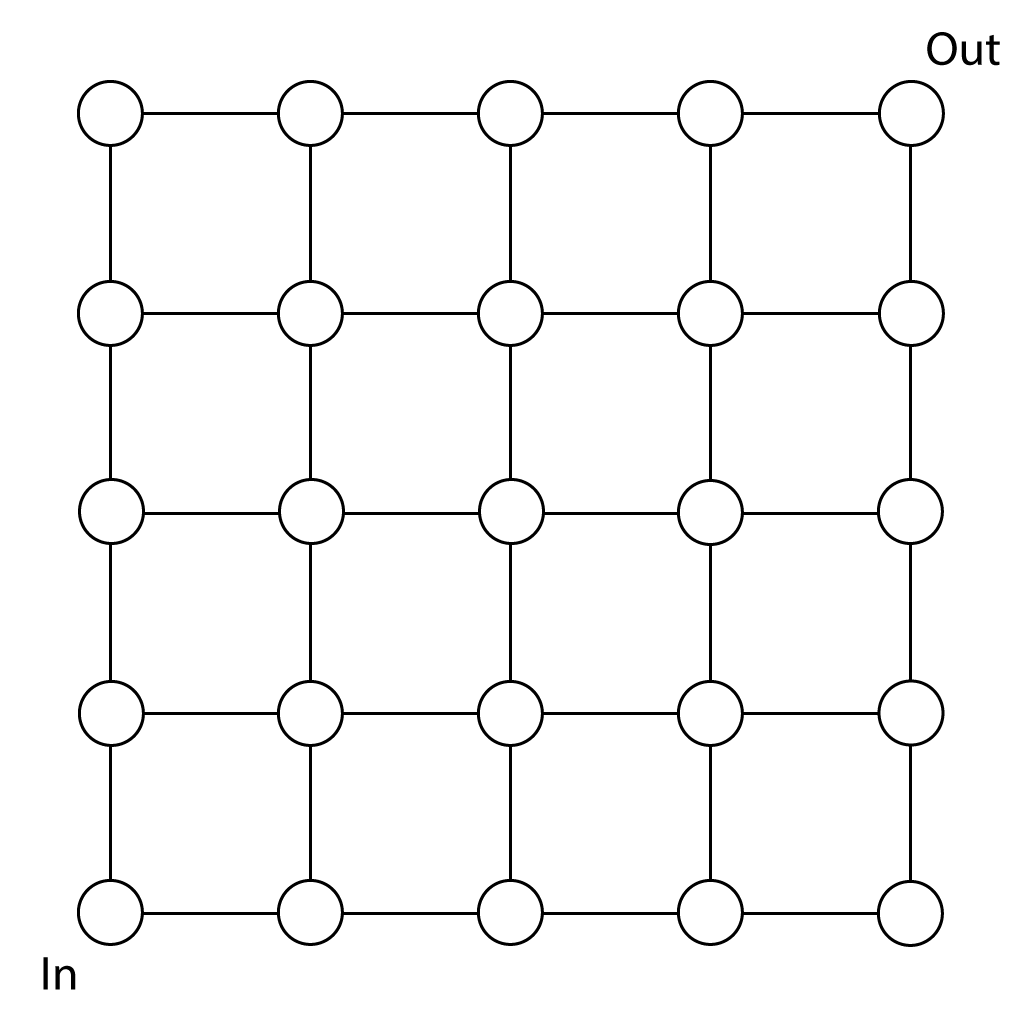
\includegraphics[width=\textwidth]{resource/grid.png}
		\caption{Fase 1: De initialisatie}
		\label{fig:lee-grid}
	\end{subfigure}
	\begin{subfigure}{0.32\textwidth}
		\centering
		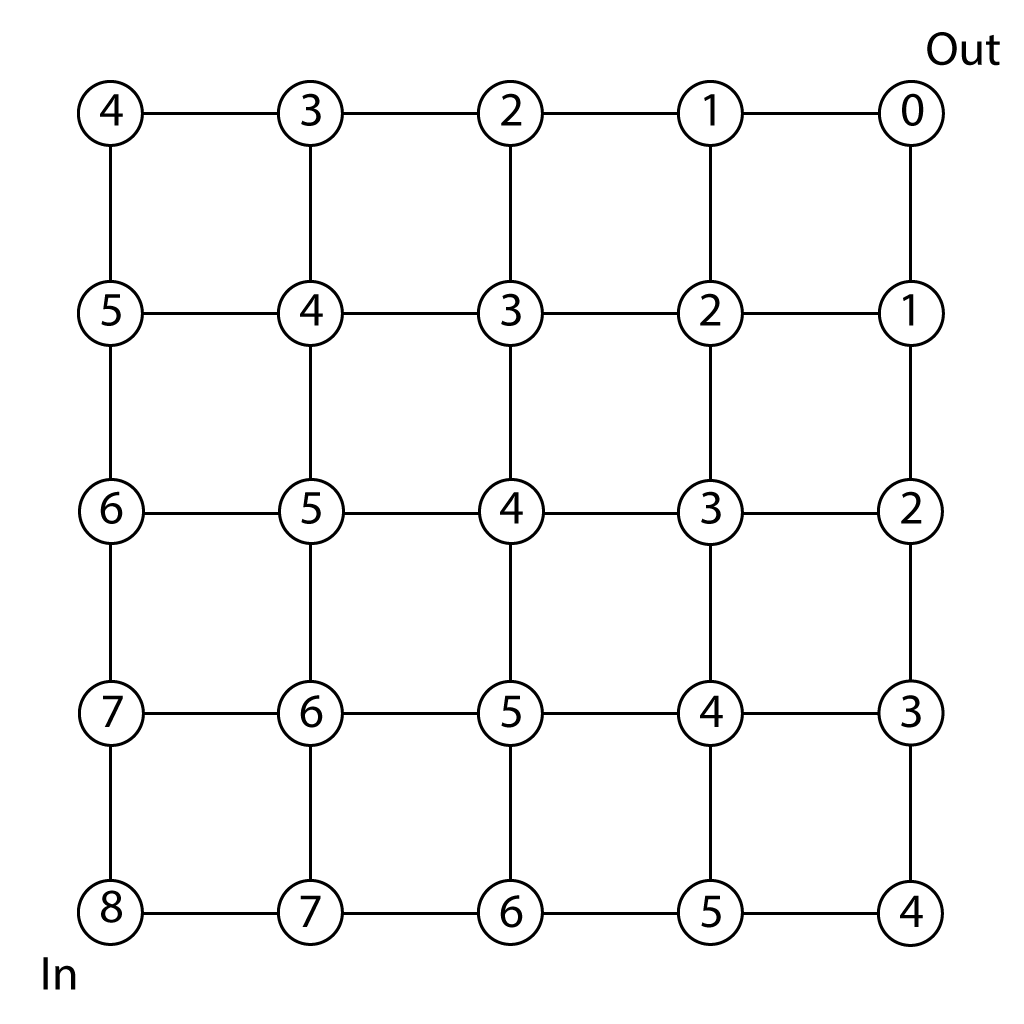
\includegraphics[width=\textwidth]{resource/wave-expansion.png}
		\caption{Fase 2: De wave-expansion}
		\label{fig:lee-wave}
	\end{subfigure}
	\begin{subfigure}{0.32\textwidth}
		\centering
		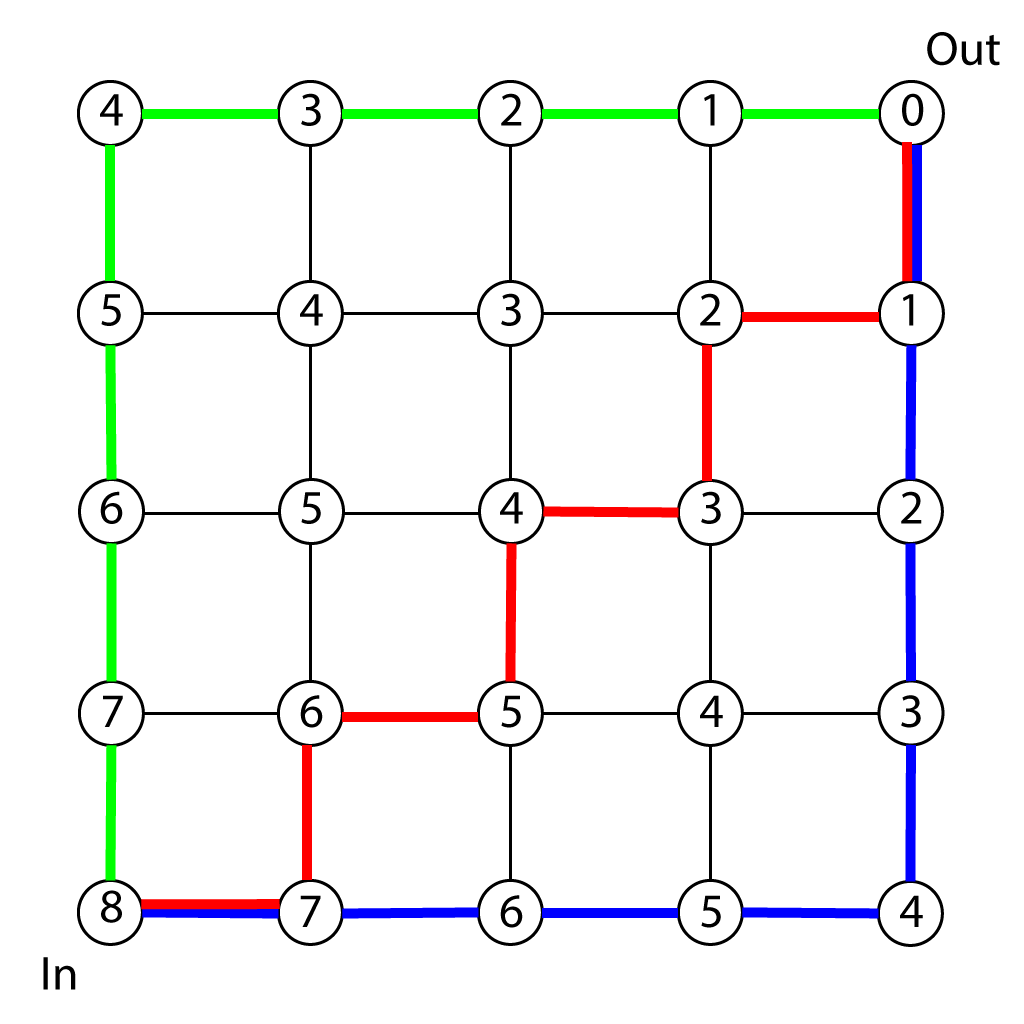
\includegraphics[width=\textwidth]{resource/path.png}
		\caption{Fase 3: De backtrace}
		\label{fig:lee-path}
	\end{subfigure}
	\caption{De drie stappen in Lee's algorithm}
	\label{fig:lee}
\end{figure}

\noindent
Lee's algoritme werkt als volgt (een schematische weergave is gegeven in figuur \ref{fig:lee}): als eerst wordt er aan elke \textit{node} (knooppunt) een waarde toegekend, beginnend bij het eindpunt.
Het eindpunt krijgt de laagste waarde, bijvoorbeeld 0.
Vervolgens krijgen alle nodes aangrenzend (niet diagonaal) aan het eindpunt een waarde 1, de nodes die op hun beurt weer grenzen aan deze nodes krijgen een waarde 2, enzovoorts.
Door het patroon wat hierdoor ontstaat heet deze fase de \textit{wave-expansion} fase.
Vervolgens begint de \textit{backtrace}; de waarde van het startpunt wordt geëvalueerd, deze is bijvoorbeeld gelijk aan 5.
Dan worden de waarden voor iedere aangrenzende node bekeken, tenminste één van deze zal een lagere waarde hebben dan het startpunt, de waarde 4, en is dus dichter bij het eindpunt.
Deze wordt dan opgenomen in het pad en zal vervolgens op dezelfde manier worden geëvalueerd.
Dit proces herhaalt zich totdat het eindpunt met waarde 0 is gevonden en het pad compleet is.
Op deze wijze zijn er een aantal mogelijkheden om tot een pad te komen dat zo kort mogelijk is, dit is zichtbaar in figuur \ref{fig:lee-path}, waar drie mogelijke paden zijn gemarkeerd in rood, groen en blauw.
De route die uiteindelijk berekend wordt, is afhankelijk van de manier waarop het algoritme geïmplementeerd wordt (hier komen we zo nog op terug).
Mijnen kunnen in Lee's algoritme ontweken worden door tijdens de wave-expansion twee aangrenzende nodes, die van elkaar gescheiden zijn door een mijn, niet mee te tellen als buren en de aangrenzende node dus op dat moment over te slaan.\\

\noindent
De op dit algoritme gebaseerde programma's waren allemaal in staat een pad te vinden over het wedstrijdveld en enkele konden hierbij ook al mijnen ontwijken.
De implementatie van Lee's algoritme voldoet hiermee in principe aan alle drie de gestelde eisen en kan gebruikt worden om de robot aan te sturen.
De berekende kortste route hoeft echter niet \textit{altijd} de snelste route te zijn.
Zo zou de door het algoritme berekende kortste route een X aantal bochten kunnen bevatten - in het geval van de rode route in figuur \ref{fig:lee-path} zijn dit er zeven -  waar een andere route, die dezelfde lengte heeft, er maar één heeft (blauw of groen in figuur \ref{fig:lee-path}.
Omdat het aannemelijk is dat de robot sneller rechtdoor rijdt dan dat hij een bocht neemt, zouden de blauwe en groene routes dus beter zijn, terwijl dit niet per se de berekende routes zijn.

Dit was voor een situatie zonder mijnen geen probleem.
Omdat het computerprogramma sequentieel is, zal het altijd een voorkeur hebben voor een bepaalde richting.
Dit is de eerste (of de laatste) richting waarvoor het programma checkt of de route er wellicht langs kan gaan.
Het gevolg hiervan is dat de route altijd slechts één bocht zal bevatten.
Wanneer we echter obstakels toe gaan voegen zou het voor kunnen komen dat het programma op een punt met twee keuzes aankomt: één voor een pad met één bocht en een ander dat bestaat uit een zigzag, beide met dezelfde lengte.
In deze situatie kan het dat het programma het zigzagpad kiest, omdat dat als eerste (of als laatste) gecontroleerd wordt.
Dit betekent niet-optimaal gedrag en moet dus voorkomen worden.
Daarom is er voor gekozen ook naar een tweede algoritme te kijken: het A*-algoritme.

\subsection{A*}
\label{ssec:astar}

Het A*-algoritme gebruikt, in tegenstelling tot dat van Lee, een bepaalde heuristiek.
Dit betekent dat er al een zekere kennis bestaat bij het bepalen
van een geschikt pad naar het doel.
Het programma ``weet'' bijvoorbeeld dat het doel boven het startpunt zit en houdt hier rekening mee bij het berekenen van het pad.
Dat levert in potentie sneller resultaat op met minder geheugengebruik.
Nu is het niet zo dat het berekenen van een pad over een grid van 5x5 een zeer intensieve taak is, maar het zijn hoe dan ook twee positieve eigenschappen.
Daarnaast kan de complexiteit van de heuristische functie gevarieerd worden - dit is de functie die berekent hoe geschikt de node is voor het pad - om een optimaal pad, met zo min mogelijk bochten en zonder tussenkomst van mijnen, te berekenen.\\

\noindent
A* begint zijn zoektocht naar het kortste pad bij het startpunt.
Vanaf het begin houdt het algoritme een \textit{openlist} bij, deze lijst bevat alle nodes die nog geëvalueerd kunnen worden en mogelijk een onderdeel van pad zijn.
Vervolgens wordt er voor elk van de \textit{aanliggende nodes} aan deze \textit{huidige node} een zogenaamde \textit{voorwaardelijke g-score} bepaald: deze score is de afstand van de aanliggende node tot het startpunt.
Omdat alle afstanden in een grid als dat van ons altijd gelijk zijn aan 1 (of een andere constante), wordt de score van een aanliggende node altijd 1 hoger dan de huidige node.
In het geval van een aanliggende node die naast het startpunt ligt is de voorwaardelijke g-score dus gelijk aan 1.
Vervolgens wordt deze voorwaardelijke g-score vergeleken met de g-score (niet voorwaardelijk) van de aanliggende node.
Wanneer de voorwaardelijke g-score van de aanliggende node lager is dan de al opgeslagen g-score of de aanliggende node zich nog niet in de openlist bevindt volgen er een aantal stappen:

\begin{enumerate}
	\item De huidige node wordt bij de aanliggende node ingesteld als \textit{vorige}, dat wil zeggen, de node ``waar je vandaan kwam''
	\item De voorwaardelijke g-score wordt bij de aanliggende node ingesteld als g-score en is dus niet langer voorwaardelijk
	\item Er wordt een \textit{h-score}, waarbij de h staat voor heuristiek, berekend voor de aanliggende node, dit is de verwachte afstand tot het eindpunt
	\item Er wordt een totale score, de \textit{f-score}, berekend voor de aanliggende node, deze score is gelijk aan de g-score + de h-score
	\item De aanliggende node wordt toegevoegd aan de openlist aan de hand van zijn f-score, hoe hoger deze is, des te verder naar achter de node wordt ingedeeld
\end{enumerate}

\noindent
Nadat dit proces zich voor ieder aanliggende node heeft herhaald (vier maal dus) zitten er dus een n-aantal nodes extra in de openlist.
Vervolgens wordt de node met de laagste f-score, het eerste item van de openlist, ingesteld als huidige node en begint het proces opnieuw.
Dit herhaalt zich totdat het eindpunt als huidige node wordt aangewezen.
Op dat moment begint net als bij het algoritme van Lee een backtrace, maar ditmaal op basis van de ''vorige''-verwijzing die in iedere node is opgeslagen.
Iedere node verwijst op die manier namelijk terug naar een andere, tot aan het startpunt.
Wanneer de hiermee opgebouwde lijst dan tot slot wordt geïnverteerd, wordt het een pad van begin tot eind.
\\

\noindent
Simpel gezegd gaat het algoritme zo hard mogelijk richting het eindpunt, waarbij het er dus op neer komt dat telkens de eerste node uit de openlist een onderdeel van het pad wordt.
Dit gaat zo door totdat er een obstakel voorkomt, in dit geval valt het algoritme terug op de laatst bekende node die nog beschikbare aanliggende nodes heeft.
Vanuit daar gaat het algoritme op dezelfde manier verder, totdat het eindpunt gevonden is.
\\

\noindent
Om mijnen te ontwijken is simpelweg een check ingebouwd, tijdens het evalueren van de aanliggende nodes; wanneer er een mijn ligt tussen de huidige en aanliggende node, wordt deze gewoon overgeslagen en kan hij dus niet aangemerkt worden als ``vorige'' en komt zo niet in het uiteindelijke pad terecht.
Het bestaan van mijnen wordt per node opgeslagen in een array.
Voor elke mogelijke richting (links, rechts, boven, beneden) is er een index die een 1 of een 0 bevat.
Ook het vermijden van bochten is gemakkelijk in gebouwd, in onze implementatie wordt tijdens het bepalen van de voorwaardelijke g-score 2 opgeteld bij de g-score, als er een bocht gemaakt moet worden om bij de desbetreffende aanliggende node te komen.
Deze hogere g-score zal dus resulteren in een node die verder naar achteren in de openlist komt te staan en daarom is het dus minder waarschijnlijk dat hij gekozen wordt als onderdeel van het pad.
\\

\noindent
De flexibiliteit en efficiëntie ten opzichte van Lee's algoritme hebben er toe geleid dat er ook nog een implementatie van het A*-algoritme is gemaakt, die inderdaad een stuk sneller is met minder geheugengebruik, uiteraard pas waarneembaar bij absurde dimensies.
Ook aan de eisen ``mijnen ontwijken'', ``mijnen opslaan'' en ``bochten vermijden'' is voldaan, dus de keuze is gevallen op A* voor verder gebruik bij het project.
De gebruikte C-implementatie is te vinden in de bijlagen onder \cite{sec:code-navigation}

\end{document}